\section{Desarrollo de un vector numérico}

\begin{frame}[t,fragile]{Objetivo}
\begin{itemize}
\item En esta unidad iremos incorporando los conceptos al desarrollo de un tipo 
      \textmark{vector numérico}: \cppid{vecnum}.
  \begin{itemize}
    \item Tipo con funcionalidad parecidad a \cppid{vector<double>}.
  \end{itemize}
\begin{lstlisting}
  vecnum v(5);
  v[2] = 3.0;
  for (int i=0; i<v.tamanyo(); ++i) {
    std::cout << "v[" << i << "] = " << v[i] << '\n';
  }
\end{lstlisting}

  \mode<presentation>{\vfill\pause}
  \item \textgood{Alternativas}:
  \begin{itemize}
    \item Usando \cppid{unique\_ptr}.
    \item Usando punteros primitivos.
  \end{itemize}

\end{itemize}
\end{frame}

\begin{frame}[t]{Usando \textbf{unique\_ptr}}
\begin{block}{vecnum.hpp}
\lstinputlisting[basicstyle=\tiny]{ejemplos/01-constr-destr/smart-vecnum/vecnum.hpp}
\end{block}
\end{frame}

\begin{frame}[t]{Usando \emph{punteros primitivos}}
\begin{block}{vecnum.hpp}
\lstinputlisting[basicstyle=\tiny]{ejemplos/01-constr-destr/primitive-vecnum/vecnum.hpp}
\end{block}
\end{frame}


\begin{frame}[fragile]{Comprobación de memoria}
\begin{itemize}
  \item \textgood{valgrind}: 
        Conjunto de herramientas para realizar análisis dinámico de programas.
    \begin{itemize}
      \item \textmark{memcheck}: Herramienta para:
        \begin{itemize}
          \item Accesos indebidos a memoria.
          \item Usos peligrosos de valores no iniciados.
          \item Goteos de memoria.
          \item Errores en liberación de memoria.
        \end{itemize}
    \end{itemize}
  \item Invocación:
\begin{lstlisting}[style=terminal]
valgrind --tool=memcheck programa
\end{lstlisting}
\begin{lstlisting}[style=terminal]
...
==15344== HEAP SUMMARY:
==15344==     in use at exit: 40 bytes in 1 blocks
==15344==   total heap usage: 1 allocs, 0 frees, 40 bytes allocated
==15344== LEAK SUMMARY:
==15344==    definitely lost: 40 bytes in 1 blocks
...
\end{lstlisting}
\end{itemize}
\end{frame}

\begin{frame}[t]{\textbf{valgrind} desde CLion}
\begin{itemize}
  \item \textmark{valgrind} está integrado en \textmark{CLion}.
    \begin{itemize}
      \item Se puede ejecutar desde \textgood{Run} | \textgood{Rin with valgrind memcheck}.
      
\includegraphics[width=2em]{images/01-constr-destr/valgrind.png}
    \end{itemize}
  \mode<presentation>{\vfill\pause}
  \item Resultado en panel de \textmark{Run valgrind memcheck}.
\end{itemize}
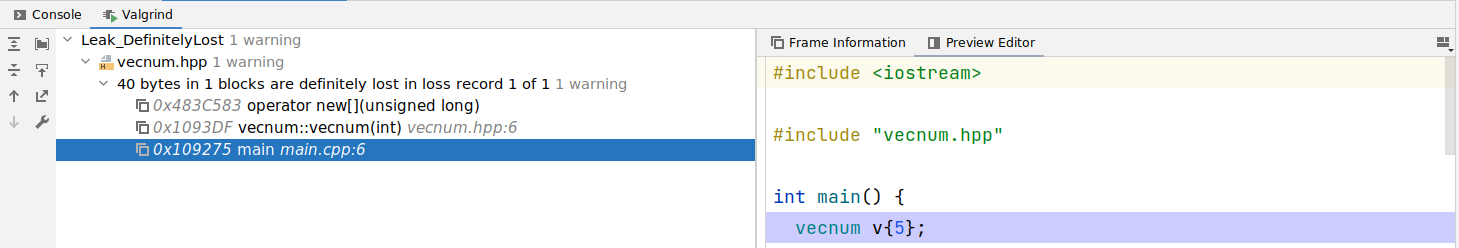
\includegraphics[width=\textwidth]{images/01-constr-destr/vecnum-main-valgrind.png}
\mode<presentation>{\vfill\pause}
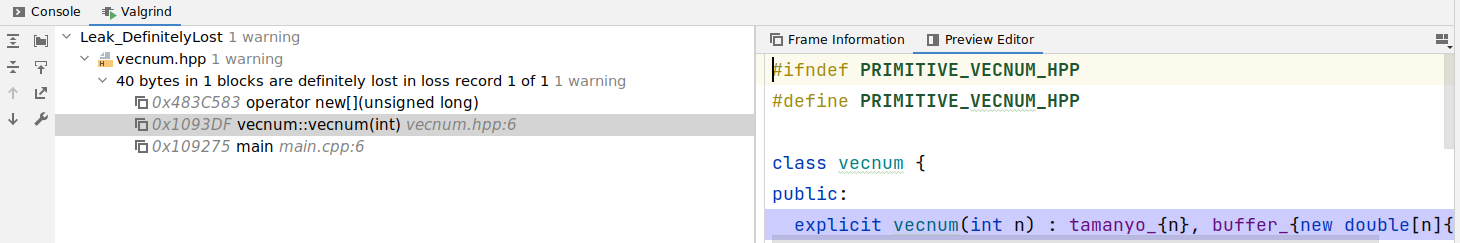
\includegraphics[width=\textwidth]{images/01-constr-destr/vecnum-ctor-valgrind.png}
\end{frame}

\begin{frame}[t]{Otra alternativa: \emph{sanitizers}}
\begin{itemize}
  \item Un \textgood{sanitizer} es una opción que instrumenta el código generado
        para detectar distintos tipos de errores.
    \begin{itemize}
      \item \textmark{AddressSanitizer}: Detecta errores de memoria.
      \item \textmark{LeakSanitizer}: Subconjunto de AddressSanitizer para goteos de memoria.
      \item \textmark{ThreadSanitizer}: Detecta errores de concurrencia.
      \item \textmark{UndefinedBehaviorSanitizer}: Detecta comportamientos no definidos.
      \item \textmark{MemorySanitizer}: Detecta acceso a memoria no iniciada (solo \textgood{clang}).
    \end{itemize}
\end{itemize}
\end{frame}

\begin{frame}[t,fragile]{Uso de \textbf{AddressSanitizer}}
\begin{itemize}
  \item Modificación de opciones de compilación y enlace.
\end{itemize}
\begin{lstlisting}
add_compile_options(-fsanitize=address -fno-omit-frame-pointer)
add_link_options(-fsanitize=address -fno-omit-frame-pointer)
\end{lstlisting}

\mode<presentation>{\vfill\pause}
\begin{itemize}
  \item Crear un perfil de ejecución en CLion.
    \begin{enumerate}
      \item Abre la ventana de \textmark{settings} del proyecto.
      \item Selecciona \textmark{Build, Execution, Deployment}.
      \item Selecciona \textmark{CMake}.
      \item Copia el perfil \textmark{Debug} en un nuevo perfil.
      \item Cambia el nombre a \textmark{Debug-address-sanitizer}.
      \item En el campo de opciones pon 
            \cppid{-DCMAKE\_CXX\_FLAGS="{}-fsanitize=address -fno-omit-frame-pointer"}.
    \end{enumerate}
\end{itemize}
\end{frame}

\begin{frame}[t,fragile]{Resultado de Address Sanitizer}
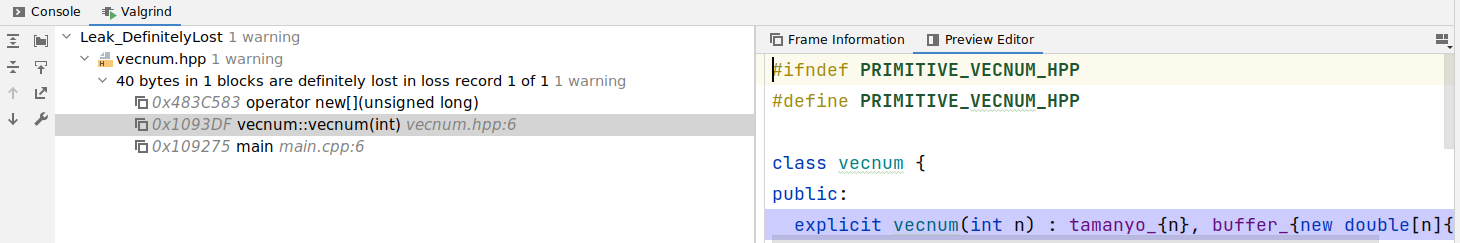
\includegraphics[width=\textwidth]{images/01-constr-destr/vecnum-ctor-valgrind.png}
\mode<presentation>{\vfill\pause}

\begin{columns}[T]
\column{.5\textwidth}
\textgood{AddressSanitizer}
\begin{itemize}
  \item Instrumentación binaria
  \item Deceleración = 2x
  \item Detecta desbordamientos
  \item No detecta accesos a memoria sin iniciar
\end{itemize}

\column{.5\textwidth}
\textgood{valgrind memcheck}
\begin{itemize}
  \item Instrumentación en compilación
  \item Deceleración = 20x
  \item No detecta desbordamientos
  \item Detecta accesos a memoria sin iniciar
\end{itemize}

\end{columns}
\end{frame}
